\chapter{Introduction}
The dominant force over large distances is the gravitational force.
It controls the motion of planets in the solar system and is responsible for the evolution of stars and galaxies, and the whole cosmos \cite{nordtvedt2025gravity}.
Although the motion of two bodies orbiting each other lends itself to an analytical description, no general solution for systems comprising three or more bodies is known.
Therefore, the importance of numerical simulations of many-body systems (usually referred to as \textit{N-body simulations}) is hard to overestimate.

Even though the direct beneficiary of advances in the area of $N$-body simulations is the field of astrophysics, the development of such tools is highly interdisciplinary in nature.
The theory behind algorithms that make fast simulations of this type possible is often involved mathematically and requires a good grasp of general physics.
On the other hand, efficient implementation of these ideas demands proficiency in computer science, particularly in areas such as data structures, parallel computing, and performance optimization.
Consequently, the development of $N$-body simulation codes is challenging but also intellectually rewarding.

\section{Problem statement}
To better understand the computational challenge before us, we begin by formulating the physical setup.
The force exerted on a body with mass $m_2$ at the point $\mathbf{x}_2$ by a body with mass $m_1$ located at $\mathbf{x}_1$ can be expressed by the relation
\begin{equation}\label{eq:law-of-uni-grav}
    \mathbf{F} = -G\frac{m_1m_2}{|\mathbf{x}_{21}|^3}\mathbf{x}_{21}
\end{equation}
where $G$ is the gravitational constant $6.674\times 10^{-11}\, \mathrm{m}^3 \,\mathrm{kg}^{-1}\,\mathrm{s}^{-2}$ and $\mathbf{x}_{21} = \mathbf{x}_2 - \mathbf{x}_1$.
Therefore, the evolution of a system of $N$ bodies is governed by $N$ equations
\begin{equation}\label{eq:pp-method}
    \ddot{\mathbf{x}}_i = -G\sum_{j\neq i} \frac{m_j}{|\mathbf{x}_{ij}|^3}\mathbf{x}_{ij}.
\end{equation}
for each $i = 1,\dots, N$.
Direct application of \autoref{eq:pp-method} is the basis of the so-called \textit{particle-particle} method.
The method is characterized by $O(N^2)$ time complexity (more precisely, it requires $(N-1)N/2$ operations if Newton's 3rd law is used in the computation).
This running time characteristic $T(N)$ (running time of one simulation iteration) can be directly observed by running an implementation of the method (see \autoref{fig:pp-method-scaling}).
\begin{figure}[htp]
    \centering
    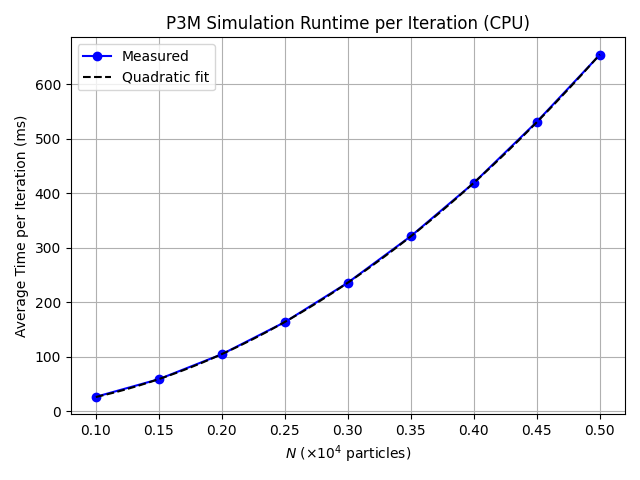
\includegraphics[scale=0.5]{chapters/introduction/img/pp_time.png}
    \caption{Scaling of the PP method.}
    \label{fig:pp-method-scaling}
\end{figure}
The exact form of $T(N)$ depends on the implementation details and the type of hardware used, but assuming that the code whose running time is shown in \autoref{fig:pp-method-scaling} is not tragically inefficient, we can draw some general conclusions regarding the applicability of the PP method.
Fitting a quadratic through the points shown in the figure reveals the following approximation: $T(1{,}000N) \approx 26.1N^2 + 0.32N$ [ms].
In a reasonable particle simulation, one often deals with tens of thousands of particles (if not more) and the simulation can span hundreds of iterations.
Thus, assuming sensible values of $N = 50{,}000$ and 200 iterations, we get the expected running time of $\approx 3.5$ hours!
This clearly shows that more efficient algorithms have to be put in place.

\section{Historical development}\label{sec:historical-development}
The \textit{particle-mesh} (PM) technique, introduced by Roger W. Hockney and James W. Eastwood, was a significant improvement over the PP method.
In the PM approach, the space is divided into a rectangular grid (or mesh) of cells.
Each cell is assigned a portion of the mass of nearby particles, creating a density distribution $\rho(\mathbf{x})$.
The relation between the density and the gravitational potential $\phi$, in the form of Poisson's equation
\begin{equation}\label{eq:poisson}
    \nabla^2\phi = 4\pi G \rho,
\end{equation}
is then used to obtain the potential at each cell center using Fourier techniques.
The gravitational field $\mathbf{g}$ can then be calculated as $\mathbf{g} = -\nabla \phi$.
Since $\mathbf{g}$ equals the acceleration due to gravity, we get $\ddot{\mathbf{x}}_i = \mathbf{g}(\mathbf{x}_i)$.
The PM method and its theoretical grounding were most extensively described by Hockney and Eastwood in \textit{Computer Simulation Using Particles} textbook published in 1988 \cite{Hockney1988}.
However, one of the first papers treating the problem of solving the Poisson equation using Fourier analysis (\textit{A Fast Direct Solution of Poisson's Equation Using Fourier Analysis} by R.W. Hockney) can be traced back to 1965 \cite{10.1145/321250.321259}.

The drawback of the PM method is its poor modeling of forces over short distances.
Eastwood and Hockney proposed a remedy for this problem in the form of a hybrid approach, called the \textit{particle-particle-particle-mesh} method (or \PThreeM{} in short).
In the \PThreeM{} method, the force on a given particle is split into two components: \textit{short-range} and \textit{long-range} force.
The long-range force is calculated using the PM method, whereas the short-range force can be found by direct summation of the forces due to nearby particles.
The \PThreeM{} method was developed across the papers published by the authors between 1973 and 1980 with its thorough description given in \textit{Computer Simulation Using Particles} \cite{Hockney1988}.

The computational complexity of the PM and \PThreeM{} methods depends on the implementation of the potential solver used to calculate $\phi$ from \autoref{eq:poisson}.
For instance, if a fast Fourier transform is used, then the complexity of the PM algorithm is $O(N + N_g^3\log N_g^3)$, where $N_g$ is the number of cells in a single dimension of the grid (note that it is linear in $N$).
For the \PThreeM{} method, the worst-case scenario happens when all particles are clustered closely together, which causes the short-range $O(N^2)$ correction part to become dominant.

In 1986, Josh Barnes and Piet Hut introduced a hierarchical method for $N$-body simulations, now known as the Barnes-Hut algorithm, in the paper \textit{A hierarchical O(N log N) force-calculation algorithm} \cite{barnes1986hierarchical}.
The method developed by the authors uses a hierarchical subdivision of space into cubical cells where the subdivision is carried out recursively until at most one body can be found in any subdivision.
The algorithm reduces the time complexity to $O(N \log N)$ by approximating groups of distant particles as a single ``pseudo-particle.''

Other notable examples of $N$-body simulation algorithms include (and are not restricted to) the Fast Multipole Method and Adaptive Mesh Refinement method \cite{trenti2008nbody}.

\section{Aim and scope}
This thesis has three main goals:
\begin{enumerate}
    \item To develop a program implementing the PM, \PThreeM{}, and Barnes-Hut algorithms focusing on correctness and performance;
    \item To introduce these algorithms and analyze their strengths and weaknesses through error analysis and performance benchmarks using our implementation;
    \item To implement simple astronomical system models to test and evaluate the methods.
\end{enumerate}
The field of $N$-body simulations has been extensively studied (see \autoref{sec:historical-development}), making novel contributions challenging.
However, since our implementation is written from scratch, we aim to provide practical insights via:
\begin{enumerate}
    \item Comparing GPU and CPU implementations of the PM method;
    \item Parallelizing the short-range correction in the \PThreeM{} method;
    \item Implementing a cache-friendly tree construction for the Barnes-Hut algorithm.
\end{enumerate}
The complete source code, including all algorithms and simulation models, is available at \url{https://github.com/AleksyBalazinski/ParticleSimulation}.
